\documentclass[10pt,twocolumn,letterpaper]{article}
\usepackage[pagenumbers]{cvpr}
\usepackage{times,graphicx,amsmath,amssymb,booktabs,multirow}
\usepackage{tikz}
\usetikzlibrary{positioning,arrows.meta,fit}
\usepackage[pagebackref,breaklinks,colorlinks,allcolors=blue]{hyperref}
\newcommand{\method}{TICK\xspace}
\newcommand{\pp}{\,\mathrm{pp}}
\newcommand{\event}{\mathcal{P}_{\mathrm{E}}}
\newcommand{\state}{\mathcal{P}_{\mathrm{SA}}}
\title{TICK: Diagnosing the Temporal--Semantic Gap\\in Brief Video Relation Recovery}
\author{Anonymous authors\\Initial manuscript}
\begin{document}
\maketitle

\begin{abstract}
Video relation detection must distinguish the persistence of an entity pair from the times at which its relations hold. A person and an object may remain visible while their interaction occurs only briefly or repeatedly. We investigate whether explicitly predicting event onsets improves brief-relation recovery while preserving long-duration relations under a finite prediction budget. Our experimental framework, TICK, combines a query-based temporal-mask branch with a predicate-conditioned onset branch and evaluates temporal matching separately from predicate-aware matching. A five-seed experimental record on 250 VidOR validation videos reveals a sharp separation between these requirements. At a cap of nine candidates per window, routing improves short-relation temporal matching by 4.02 percentage points but reduces predicate-aware matching by 1.69 points for short relations and 5.81 points for long relations. Classification, ranking, and temporal re-anchoring variants do not resolve the trade-off. Ground-truth-interval classification further shows limited semantic recovery in the tested small-sample setting. The central finding is a temporal--semantic gap: improved interval coverage does not translate into correctly labeled brief relations in this onset-routing framework. These results motivate joint evaluation of event timing, semantic assignment, and the preservation of long-duration relation predictions.
\end{abstract}

\section{Introduction}
Video visual relation detection represents a video as relations between specific entities over time. Its output is not merely a list of objects and predicates, but a set of subject--predicate--object instances with temporal support~\cite{shang2017video,shang2019annotating}. This distinction is essential for understanding interaction. Two people may remain in the scene for almost a minute, while one looks at the other only during several brief episodes. A useful prediction must identify the participants, name the relation, and recover each interval during which that relation is annotated to hold.

Existing methods address both semantics and time. BIG first predicts relational triplets and then grounds their temporal instances~\cite{gao2022classification}. VrdONE instead formulates relation prediction as one-dimensional instance segmentation over entity-pair features, jointly predicting predicate categories and temporal masks~\cite{jiang2024vrdone}. These approaches provide a foundation for continuous video understanding. They also motivate a finer question: when the entities remain available, how reliably does a model isolate the brief occurrences of their relations?

Figure~\ref{fig:case} illustrates the difficulty in a real VidOR video. The two annotated entities coexist for 57.29 seconds and have eight separate \emph{watch} annotations. A high-scoring VrdONE prediction spans 43.68 seconds, including a highlighted event lasting only 1.13 seconds. The temporal overlap with that individual event is small despite the prediction naming the relevant predicate and covering its time. The full timeline matters: the prediction overlaps several occurrences, and the error cannot be represented faithfully by drawing only a single short annotation. This example motivates \emph{event-level temporal support within a persistent entity pair}.

An attractive response is to replace extended masks with explicit event onsets. A point-like onset target emphasizes when a relation starts; a duration estimate converts the detected point into an interval. Related temporal action localization methods already demonstrate the value of temporal scale modeling and explicit boundaries~\cite{zhao2021video,zhang2022actionformer,shi2023tridet}. For video relations, however, recovering a compact interval is only part of the task. The interval must be assigned to the correct predicate and participants, and its candidate must survive selection alongside persistent relations. A change that produces more temporally plausible intervals can therefore improve a timing diagnostic while worsening the relation output.

We study this distinction using \method, a two-branch experimental framework (Figure~\ref{fig:overview}). A VrdONE-style query branch predicts temporal masks, while an onset branch predicts candidates for a designated set of Event predicates. Motivated by persistent-pair examples, we evaluate all short-duration relations in the available subset; the experimental record does not supply a persistent-pair-conditioned aggregate. We compare the branches and their combinations under a common per-window candidate cap, separately recording temporal and predicate-aware matching. The study includes a disjoint-video reevaluation, alternative interval decoders, predicate competition, cross-branch ranking, temporal re-anchoring, and a classifier operating on ground-truth event intervals.

The main router improves short-interval temporal matching, but this gain does not establish better relation detection. Under a cap of nine candidates, routing reduces predicate-aware short-relation performance and sacrifices long-duration relations. Adding class competition, calibrating branch ranks, or transferring onset times to query predictions does not produce the desired joint improvement. These outcomes focus the research problem on the connection between localized evidence, relation semantics, and output selection.

Our contributions are threefold. First, we establish an onset--mask comparison framework that separates temporal readout, predicate agreement, and candidate budget. Second, we identify a divergence between short-interval gains and semantic and long-relation losses under a common output cap. Third, decoding, ranking, re-anchoring, and ground-truth-interval probes characterize the parts of brief-relation recovery that remain unresolved by the tested framework.

\begin{figure}[t]
\centering
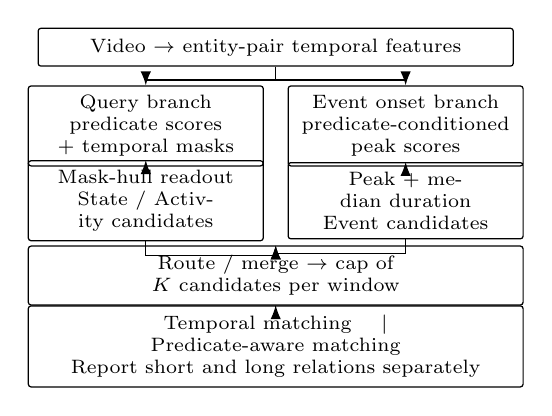
\begin{tikzpicture}[font=\scriptsize,>=Latex,
 box/.style={draw,rounded corners=1pt,align=center,minimum height=0.48cm,text width=2.75cm},
 every path/.style={line width=0.45pt}]
\node[box,text width=5.8cm] (input) at (0,0) {Video $\rightarrow$ entity-pair temporal features};
\node[box] (q) at (-1.65,-1.0) {Query branch\\predicate scores + temporal masks};
\node[box] (e) at (1.65,-1.0) {Event onset branch\\predicate-conditioned peak scores};
\node[box] (h) at (-1.65,-1.95) {Mask-hull readout\\State / Activity candidates};
\node[box] (p) at (1.65,-1.95) {Peak + median duration\\Event candidates};
\node[box,text width=6.05cm] (k) at (0,-2.9) {Route / merge $\rightarrow$ cap of $K$ candidates per window};
\node[box,text width=6.05cm] (m) at (0,-3.8) {Temporal matching \quad $\vert$ \quad Predicate-aware matching\\Report short and long relations separately};
\draw[->] (input.south) -- ++(0,-0.17) -| (q.north);
\draw[->] (input.south) -- ++(0,-0.17) -| (e.north);
\draw[->] (q) -- (h); \draw[->] (e) -- (p);
\draw[->] (h.south) -- ++(0,-0.18) -| (k.north);
\draw[->] (p.south) -- ++(0,-0.18) -| (k.north);
\draw[->] (k) -- (m);
\end{tikzpicture}
\caption{\textbf{Experimental framework.} \method compares mask-based and onset-based outputs while tracking their semantic validity and competition for a finite output budget. Event denotes a predicate category group, not a duration bin. The short-relation evaluation uses duration independently of that grouping.}
\label{fig:overview}
\end{figure}

\begin{figure*}[t]
\centering
\includegraphics[width=\textwidth]{figures/figure2_case.pdf}
\caption{\textbf{A brief relation within a persistent entity pair.} VidOR validation video \texttt{1018\_4199369046}, subject \#3 and object \#4. The full timeline shows their 57.29-second co-presence, a persistent \emph{next\_to} annotation, and all eight \emph{watch} occurrences. The highest-scoring saved VrdONE candidate for the mapped pair and \emph{watch} covers 7.34--51.02 seconds. The highlighted annotation lasts 1.13 seconds; its tIoU with the full, unclipped 43.68-second prediction is 0.026. The frames and bars use actual annotations and saved predictions. Boxes identify annotated entities for visualization; the prediction uses native proposals.}
\label{fig:case}
\end{figure*}

\section{Related Work}
\paragraph{Video relation detection.}
The original VidVRD formulation combines entity trajectories with temporally bounded relational triplets~\cite{shang2017video}. VidOR extends relation annotation to user-generated videos~\cite{shang2019annotating}. Early and subsequent methods differ in how they organize temporal context: Liu et al. use multiscale sub-tracklets and spatiotemporal graphs~\cite{liu2020beyond}; BIG separates triplet classification from multi-instance temporal grounding~\cite{gao2022classification}; and VrdONE jointly predicts predicate classes and temporal masks~\cite{jiang2024vrdone}. Thus, temporal localization, repeated relation instances, and semantic--temporal decomposition already have established precedents. Our focus is the empirical interaction between brief-event readout, predicate assignment, and a bounded candidate set.

\paragraph{Short actions and temporal boundaries.}
Temporal action localization provides related tools for resolving brief events. VSGN temporally magnifies clips and exchanges information across scales to improve short-action localization~\cite{zhao2021video}. ActionFormer uses a multiscale temporal feature pyramid and predicts action categories and boundary distances at temporal locations~\cite{zhang2022actionformer}. TriDet estimates relative boundary distributions and aggregates temporal information at different granularities~\cite{shi2023tridet}. These works motivate studying the temporal support of short video relations, but action localization results do not establish gains for entity-specific relation triplets. Our comparisons ask whether a timing improvement survives the additional semantic requirements of relation prediction.

\section{Problem and Diagnostic Design}
\subsection{Persistent entities, transient relations}
Let a video contain subject and object trajectories $\tau_s$ and $\tau_o$. A relation instance is
\begin{equation}
 r=(s,p,o,I),\qquad I=[t_b,t_e),\quad d=t_e-t_b,
\end{equation}
where $p$ is the predicate and $I$ is its annotated temporal support. An entity pair may coexist for much longer than $I$, and the same predicate can occur in several separated intervals. The pair can also have an additional persistent predicate. The case analysis preserves these distinct temporal structures, while the quantitative study stratifies relation instances by duration.

Duration makes a fixed boundary error relatively expensive. For a ground-truth interval of length $d$ and a prediction with the same start but excess duration $\delta>0$, temporal IoU is
\begin{equation}
 \operatorname{tIoU}=\frac{d}{d+\delta}.
 \label{eq:stretch}
\end{equation}
This elementary property explains why absolute timing errors require duration-sensitive analysis. It does not identify which component produced the error. In Figure~\ref{fig:case}, the interval lengths are 34 and 1,309 frames, so the highlighted event has tIoU $34/1309\approx0.026$ with the full prediction. The long prediction overlaps multiple annotations; this observation is evidence of poor event separation in this case, not proof that a persistent predicate suppresses another predicate.

\subsection{Two distinct notions of success}
We use the experiment record's two diagnostic readouts. \textbf{Temporal matching} asks whether a predicted interval matches an annotated interval under the diagnostic evaluator, ignoring the predicted predicate. \textbf{Predicate-aware matching} additionally requires the predicate to agree. These scores answer different questions: the first measures candidate temporal support, whereas the second tests whether that support carries the required relational label.

The study reports the diagnostic scores rather than official VidOR detection mAP or Recall@K. Official relation detection further constrains the subject and object categories and their spatiotemporal trajectories~\cite{shang2017video,jiang2024vrdone}. Consequently, temporal matching cannot be substituted for relation detection accuracy. We also keep the per-window candidate cap $K$ separate from video-level benchmark Recall@K.

All numerical tables below are transcribed from the supplied experimental record: detector comparisons summarize five paired seeds, whereas probe repetition statistics are unspecified. The record supplies the temporal/predicate distinction, candidate caps, and paired differences, but not the evaluator's exact overlap threshold, matching assignment, or window aggregation implementation. These diagnostics therefore retain their recorded labels; we do not reconstruct an official benchmark score from them. Original per-seed predictions and the evaluator remain required for a reproducible submission.

\subsection{Candidate budget and preservation}
Adding an event branch can increase the number of opportunities to match a ground-truth interval. We therefore use $K=9$ as the principal per-window cap and report actual candidate totals when available. A common cap constrains output size without implying identical realized counts: filtering and the number of valid events can leave different methods below the cap. The $K=18$ results are budget-sensitivity analyses with larger realized outputs than $N$, rather than candidate-count-matched headline comparisons.

Short and long relations are evaluated together. The experiment record defines short relations as $d\leq2$ seconds and treats the remaining relations as long. This operational split differs from the semantic Event partition used by the architecture. An Event predicate can have a long occurrence, and a State or Activity predicate can have a short one. We do not treat the Event branch's short-relation match rate as accuracy on an unreported Event--short intersection.

The recorded acceptance criterion requires at least a three-percentage-point short-relation improvement over the matched fine-tuning baseline, a paired confidence interval excluding zero, and less than one point of degradation on long relations. This joint criterion expresses the research objective: recovering brief relations while retaining long-duration relations.

\section{TICK: Onset and Mask Readouts}
\subsection{Query-based relation branch}
For an entity-pair feature sequence $Z_{so}=(z_1,\ldots,z_T)$, the baseline produces query-wise predicate scores and temporal mask probabilities. VrdONE uses nine relation queries per entity pair~\cite{jiang2024vrdone}. In the public VrdONE reference implementation, the interval decoder takes the first and last positions whose mask probability exceeds 0.5. Writing the positive set as $\mathcal{A}_q$, the resulting hull is
\begin{equation}
 I_q=[\min\mathcal{A}_q,\max\mathcal{A}_q]
\end{equation}
before mapping feature positions to video coordinates and applying implementation-specific filtering. Disconnected positive positions can therefore be represented by one continuous span. This describes the decoder's operation; whether such spans account for a particular error must be established from its predictions.

\method retains this branch for a designated 26-predicate State/Activity group. The original query output is also evaluated independently as a baseline and as a control after fine-tuning the joint model. Nine queries refer to the pair-level model configuration, not a universal limit of nine relations per video.

\subsection{Predicate-conditioned event onsets}
A second head provides onset scores for the designated Event predicates,
\begin{equation}
 h_p(t)=\sigma\big(g_{\theta,p}(Z_{so})_t\big),
 \qquad p\in\event.
\end{equation}
Each Event annotation supervises a Gaussian target centered at its onset, and an onset focal objective trains these responses. The implementation uses a clipped duration-dependent target width. Its conversion between duration, heatmap indices, and video coordinates requires the original configuration; physical-time token counts are not inferred from the stride summary.

At inference, local heatmap maxima above 0.05 become onset candidates. For a peak at $\hat t$ and predicate $p$, the median-duration decoder constructs
\begin{equation}
 \hat I_{p,\hat t}=[\hat t,\hat t+\widetilde d_p),
 \label{eq:peak}
\end{equation}
where $\widetilde d_p$ is the predicate's empirical median duration. The reported implementation estimates these medians using 585 VidOR validation videos outside the 250-video evaluation subset. These labels are auxiliary development information, not training-split-only statistics. Same-class temporal NMS uses IoU 0.5, and the Event branch admits at most nine candidates per window before the final readout cap.

The branch defines a particular relation-time representation: evidence for an onset plus a predicate-dependent duration prior. It does not learn an explicit offset endpoint in this configuration. To inspect this choice, the decoding study compares peak-plus-median output with mask-hull output from the same trained Event head and with a ground-truth-duration substitution probe. The latter uses annotation information and is diagnostic rather than deployable inference.

\subsection{Routing and competing candidates}
The standard router combines State/Activity query candidates and Event onset candidates, then applies the recorded candidate cap. A quota variant allocates $K/3$ slots to Event candidates. Event-only and State/Activity-only readouts expose each branch's behavior. These alternatives distinguish the supply of short temporal candidates from their interaction with query predictions.

We additionally study three modifications from the experimental record. \textbf{Predicate competition (E1)} retains onset supervision and adds a 24-way softmax cross-entropy term at annotated Event onsets with weight 1.0. It also uses fourfold Event-window oversampling and class balancing. \textbf{Unified ranking (E2)} rank-calibrates scores within each branch, merges the candidates, and optionally applies cross-type temporal NMS at IoU 0.5 before taking the top $K$. \textbf{Re-anchoring (E3)} retains the predicate and participants of a query candidate but reconstructs its interval from an Event onset. Same-predicate and any-predicate peak variants test different correspondence constraints.

These interventions evaluate concrete ways of connecting the onset branch to the relation output. E1 changes both training supervision and sampling, whereas E2 and E3 change output construction.

\section{Experiments}
\subsection{Setup and evidence scope}
The evaluation subset, \texttt{val\_select}, contains 250 VidOR validation videos with 5,518 short and 11,469 long annotated relations. The disjoint-video reevaluation uses a collection named \texttt{train\_select}: 180 training videos, reported as non-overlapping with the 250 evaluation videos, with 89,764 frames, 869 short relations, and 213 Event annotations. The original split manifest is not supplied, so we refer to this collection by name rather than asserting that its name certifies official-training-split provenance.

The detector fine-tuning comparisons use five paired random seeds, 100--104, and 500 fine-tuning steps. The reported base learning rate is $3\times10^{-4}$ and the Event-head rate is $10^{-3}$. The main comparator $N$ is fine-tuned for the same number of steps without the additional head; $C0$ is the unmodified pretrained checkpoint. We report the paired 95\% intervals where the record provides them. They summarize the recorded seed comparisons; they are not presented as confidence intervals over arbitrary videos or datasets. All reported deltas remain attached to their own experiment's baseline. In particular, the overview baseline and the B4 decoding baseline have different recorded means and are not used interchangeably.

An earlier A5 evaluation fine-tuned on 80\% of the same 250 videos subsequently evaluated, allowed additional candidates, and used temporal-only matching. Its apparent short-relation gain of 8.75 points is excluded from the main evidence. The disjoint-video reevaluation below replaces that result as the basis for interpreting the framework. Preliminary A2, A4, and Tversky-loss variants likewise did not satisfy the recorded acceptance criterion; we do not use their failures to infer a unique architectural cause.

\subsection{Does routing improve brief relations?}
Table~\ref{tab:clean} shows the disjoint-video comparison at $K=9$. The standard router improves short-relation temporal matching by 4.02 points, with a paired interval of $[2.24,5.80]$. It simultaneously reduces long-relation matching by 6.02 points. Reserving fewer Event slots reduces the long-relation loss to 4.16 points, while retaining a 3.30-point short temporal gain. Neither meets the joint short-improvement/long-preservation criterion.

\begin{table}[t]
\centering\small
\setlength{\tabcolsep}{3pt}
\begin{tabular}{lrr}
\toprule
Readout & Short $\Delta$ (pp) & Long $\Delta$ (pp)\\
\midrule
Query control & $-0.04$ & $-0.51$\\
 & $[-1.50,1.43]$ & $[-2.10,1.07]$\\
Router & $+4.02$ & $-6.02$\\
 & $[2.24,5.80]$ & $[-8.49,-3.54]$\\
Router, Event quota & $+3.30$ & $-4.16$\\
 & $[1.68,4.93]$ & $[-6.44,-1.89]$\\
Event only & $+6.64$ & $-42.33$\\
 & $[5.05,8.24]$ & $[-42.93,-41.73]$\\
State/Activity only & $-0.11$ & $-0.74$\\
 & $[-1.56,1.33]$ & $[-2.41,0.94]$\\
\midrule
Router, predicate-aware & $-1.69$ & $-5.81$\\
\bottomrule
\end{tabular}
\caption{\textbf{Temporal gains and semantic losses at $K=9$.} Differences from the paired fine-tuning baseline $N$. Rows use temporal matching except the final predicate-aware row, for which only point estimates are supplied. Brackets give reported 95\% intervals. Event is a semantic branch; Short and Long are duration groups.}
\label{tab:clean}
\end{table}

The semantic requirement reverses the short-group conclusion. The same reevaluation records a 1.69-point decrease in predicate-aware short-relation matching for the router, together with a 5.81-point decrease for long relations. Thus, its temporal gain cannot be reported as a gain in correctly labeled relations. Its recorded candidate total is 56,159, compared with 55,771 for $N$; the quota router produces 55,718. These totals also show why a common upper cap is not an assertion of identical candidate counts.

At $K=18$, larger temporal gains occur alongside approximately 1.9 times as many candidates in the reported comparison. Predicate-aware gains remain near zero. This behavior makes output budget a necessary part of the result, rather than an implementation detail to omit when presenting recall-like measurements.

\subsection{What changes when the interval decoder changes?}
Table~\ref{tab:decode} compares decoding rules in the B4 study. The Event-only peak-plus-median decoder matches 17.93\% of short-duration ground truths under temporal-only evaluation, whereas the query baseline matches 11.29\%. This improvement accompanies a large long-group decrease, from 50.36\% to 8.04\%. The routed decoder partially retains the long branch, but its long score is still 44.35\%.

\begin{table}[t]
\centering\small
\setlength{\tabcolsep}{3pt}
\begin{tabular}{lrrr}
\toprule
Decoder & Short (\%) & Long (\%) & Cand./win.\\
\midrule
$N$: query hull & 11.29 & 50.36 & 8.94\\
Event: hull & 0.49 & 1.42 & 0.10\\
Event: peak + median & 17.93 & 8.04 & 8.09\\
Event: peak + GT duration & 17.96 & 8.14 & 8.09\\
Router: peak + median & 15.31 & 44.35 & 9.00\\
Router: Event quota & 14.59 & 46.20 & 8.93\\
\bottomrule
\end{tabular}
\caption{\textbf{B4 decoding study.} Five-seed mean diagnostic temporal match rates at $K=9$. GT-duration substitution uses annotation information. The candidate-count difference between Event hull and peak decoding prevents interpreting this table as a shape-only intervention.}
\label{tab:decode}
\end{table}

Applying mask-hull decoding to the onset-trained Event head yields a short score of 0.49\% and only 0.10 candidates per window. Peak decoding produces 8.09 candidates per window. This contrast demonstrates the importance of the full readout configuration for this head; it does not isolate interval geometry from candidate generation or establish that the baseline mask representation is the universal cause of brief-relation errors.

Replacing median duration with ground-truth duration changes the short mean from 17.93\% to 17.96\%, a difference of 0.03 points. This substitution probe produces a small point-estimate change; no uncertainty estimate for the difference or detailed substitution assignment is supplied.

The Event-only output's predicate-aware short match rate is approximately 0.3\%. Together with Table~\ref{tab:decode}, this exposes a substantial separation between matching temporal support and attaching the correct predicate to that support.

\subsection{Can semantics, ranking, or re-anchoring close the gap?}
Table~\ref{tab:interventions} compares the three follow-up interventions using the reported paired differences. E1 introduces explicit predicate competition and increases Event sampling. Its router retains a temporal short gain of 3.99 points but decreases predicate-aware short matching by 1.56 points. Long predicate-aware matching decreases by 5.85 points. The Event-only predicate-aware short score remains approximately 0.26\%. This training package does not provide a successful semantic bridge for the onset candidates.

\begin{table*}[t]
\centering\small
\setlength{\tabcolsep}{5pt}
\begin{tabular}{llrrr}
\toprule
Intervention / readout & Matching & Short $\Delta$ (pp) & Long $\Delta$ (pp) & Candidates: method / $N$\\
\midrule
E1: predicate competition, router & Temporal & $+3.99\ [1.94,6.04]$ & $-6.11\ [-8.11,-4.12]$ & Not reported\\
E1: predicate competition, router & Predicate-aware & $-1.56\ [-2.59,-0.54]$ & $-5.85\ [-6.52,-5.17]$ & Not reported\\
\midrule
E2: calibrated ranking + NMS & Temporal & $+7.07\ [5.86,8.28]$ & $-12.66\ [-14.22,-11.10]$ & 46,963 / 55,771\\
E2: calibrated ranking + NMS & Predicate-aware & $-4.31\ [-5.15,-3.48]$ & $-18.71\ [-19.21,-18.22]$ & 46,963 / 55,771\\
\midrule
E3: same-predicate re-anchoring & Temporal & $-0.04\ [-1.37,1.30]$ & $-1.62\ [-3.31,0.07]$ & 48,542 / 55,771\\
E3: same-predicate re-anchoring & Predicate-aware & $-0.45\ [-1.39,0.49]$ & $-1.12\ [-1.98,-0.26]$ & 48,542 / 55,771\\
\bottomrule
\end{tabular}
\caption{\textbf{Three attempts to connect localized events to relation outputs.} All rows use the recorded disjoint-video protocol with $K=9$ and five paired seeds. Each delta uses its experiment's matched $N$ comparator. No variant provides the joint short-relation improvement and long-relation preservation required by the study.}
\label{tab:interventions}
\end{table*}

E2 tests whether cross-branch ranking can preserve useful candidates. Rank calibration with NMS increases temporal short matching by 7.07 points, but decreases predicate-aware short matching by 4.31 points and long matching by 18.71 points. Calibration without NMS also harms both predicate-aware duration groups. The improvement of a timing score is therefore compatible with a substantial degradation of labeled output under the tested ranking rule.

E3 keeps query semantics and changes the temporal anchoring. The same-predicate variant has a temporal short difference of $-0.04$ points with an interval spanning zero; its predicate-aware difference is $-0.45$ points. Long performance decreases, and the output count falls from 55,771 to 48,542. Any-predicate anchoring produces similar reported means. Re-anchoring consequently offers no supported short-group gain in this setting. Because candidate coverage also changes, the result does not by itself prove that query semantics, rather than correspondence or interval construction, are the sole failure source.

\subsection{Predicate evidence inside ground-truth intervals}
We next examine a classification probe in which the temporal interval is supplied by annotation. The probe mean-pools subject and object ROI features within each ground-truth interval and optionally adds entity-category embeddings. It classifies the 24 designated Event predicates, comparing visual features with a conditional predicate prior and category-only input. This setup removes interval prediction from the probe, but retains the effects of finite training data, feature choice, and classifier fitting.

The recorded training set contains 207 Event instances spanning 22 of the 24 classes; evaluation contains 734 instances. This is a distinct accounting from the 213 Event annotations reported for the fine-tuning collection. The source summary does not identify the six-instance count discrepancy or give the probe split manifest, so the probe is kept separate from the 250-video detector tables.

\begin{table}[t]
\centering\small
\setlength{\tabcolsep}{5pt}
\begin{tabular}{lrr}
\toprule
Ground-truth-interval classifier & Top-1 (\%) & Top-5 (\%)\\
\midrule
Prior $P(p\mid s,o)$ & 13.1 & 39.5\\
MLP: visual features + categories & 18.0 & 59.7\\
MLP: visual features only & 17.3 & 50.5\\
MLP: categories only & 10.9 & 33.7\\
Logistic regression: visual only & 14.7 & 50.5\\
\bottomrule
\end{tabular}
\caption{\textbf{Classification with annotated intervals.} Reported probe accuracies using 207 training and 734 evaluation Event instances. These are predicate classification scores, not relation detection or detector recall. No variability estimates are supplied for this probe.}
\label{tab:probe}
\end{table}

The best recorded classifier achieves 18.0\% top-1 accuracy and 59.7\% top-5 accuracy (Table~\ref{tab:probe}). Its reported top-1 accuracy exceeds the conditional prior by 4.9 points. Visual-only features also exceed the prior's top-1 point estimate. Thus, the tested visual representation provides usable category information in this small-sample probe, but the resulting classifier is far from consistently selecting the correct Event predicate. Ground-truth timing alone does not make classification accurate in this configuration.

The probe does not measure an information-theoretic limit of the features. Mean pooling can discard within-event dynamics, the training sample is small, two classes are absent from training, and no probe uncertainty is reported. These factors remain distinct explanations for the observed accuracy. The practical observation is narrower: the tested interval feature/classifier combination is not yet a reliable source of Event labels for the routed detector.

\section{Discussion and Conclusion}
\paragraph{Architectural implications.}
An event representation should bind each localized occurrence to discriminative relation evidence and make its score comparable with query predictions. Interval-conditioned semantic representations and selection rules that retain useful query candidates are concrete design hypotheses motivated by the observed trade-off.

\paragraph{Scope.}
The quantitative study covers one 250-video VidOR subset and report-defined diagnostic matching. It does not provide official mAP, external detector comparisons, or an independent dataset result. The persistent-pair phenomenon is illustrated with an audited video, while the new quantitative tables concern all short-duration relations; a separate aggregate estimate for long-coexistence pairs is not supplied in this record. Duration priors use disjoint validation labels, and the training and probe manifests require recovery. The mechanism by which persistent context affects brief events remains open: coexistence, semantic competition, feature quality, and decoder behavior cannot be collapsed into a single proven suppression cause.

\paragraph{Conclusion.}
\method studies brief video relations through onset-based temporal output, a query-based mask branch, and controlled readout comparisons. Its experiments reveal a gap between temporal recovery and semantic recovery: generating more useful short intervals does not suffice to improve correctly labeled relations under a bounded output budget. Predicate-aware evaluation and long-duration relation preservation expose this gap, while the ground-truth-interval probe shows the limited performance of the tested small-sample semantic classifier. A method for brief relations should close all three parts of the loop---temporal support, semantic assignment, and candidate retention---within a common evaluation protocol.

\section*{LLM Usage Statement}
OpenAI ChatGPT/Codex was used to organize the supplied experimental report, draft and revise prose, check references, prepare LaTeX, and conduct internal claim--evidence reviews. The reported experimental values were retained from the source record. No missing measurements were generated. Experimental results and interpretation remain the responsibility of the human authors.

{\small
\bibliographystyle{IEEEtranN}
\bibliography{references}
}
\end{document}
